\documentclass[a4paper, 12pt]{article}
% A4纸张,article类型
\usepackage[UTF8]{ctex}
%以此支持中文
\usepackage{graphicx}
%以此插入图片
\usepackage{url}
%支持使用 \url命令
\usepackage{float}
\usepackage{xcolor}
\usepackage{hyperref} % 加载hyperref宏包 
\usepackage{listings}  % 代码高亮包
\usepackage{amsmath}
\usepackage{verbatim}

\begin{document}
  \title{第四节课实验报告}
  \author{王书一 \\ 23020007119}
  \date{September 13, 2024}
  \maketitle

 \pagenumbering{arabic}
 \tableofcontents
 \newpage
 \pagenumbering{arabic}
 %目录

  
  \section{实验目的}
1. Linux 命令行工具调试及性能分析
   - 学习如何使用 Linux 下的命令行工具(如 `gdb`、`pdb`、`strace`、`perf` 等)进行程序的调试和性能分析。
   - 掌握如何通过命令行工具识别和解决程序中的错误和性能瓶颈,优化程序运行效率。

2. 元编程演示实验
   - 探索元编程的概念及其在 Python 或 C++ 等编程语言中的应用。
   - 学习如何编写动态生成代码、提高代码可复用性与可扩展性,理解编译时与运行时的代码生成技术。

3. PyTorch 实验
   - 学习使用 PyTorch 构建和训练神经网络模型。
   - 掌握 PyTorch 张量运算、自动微分和 GPU 加速等核心功能,理解其在深度学习中的应用。
这些实验的目标是提升对调试、性能优化、代码生成及深度学习框架的理解和应用能力。
  
\section{实验环境}
\begin{itemize}
    \item 操作系统:Ubuntu 20.04
   \item 编程语言:Python 3.12.0
\end{itemize}

\section{ Linux 命令行工具调试及性能分析}

\subsection{打印调试法与日志}


写一个简单的 Python 日志记录器示例,支持不同的日志格式和选项,比如原始输出、格式化输出、基于日志级别的输出以及带颜色的输出。我们可以使用 Python 的 logging 模块和 argparse 来解析命令行参数。

\begin{itemize} 
    \item \texttt{./logger.py raw}    原始输出
    \item \texttt{./logger.py log}   格式化输出   
    \item \texttt{./logger.py ERROR}   仅显示 ERROR 及以上级别的日志 
    \item \texttt{./logger.py log color}       带颜色的输出
\end{itemize}

遇到的问题:
在编写代码中出现无法识别import命令,
后来发现是代码的shebang写错了
原因是虚拟机的python环境是2.7
\begin{figure}[H]
  \centering
    
\includegraphics[width=0.9\linewidth]{1.png}
  \caption{Python 日志记录器}
   \end{figure}

\begin{figure}[H]
  \centering
    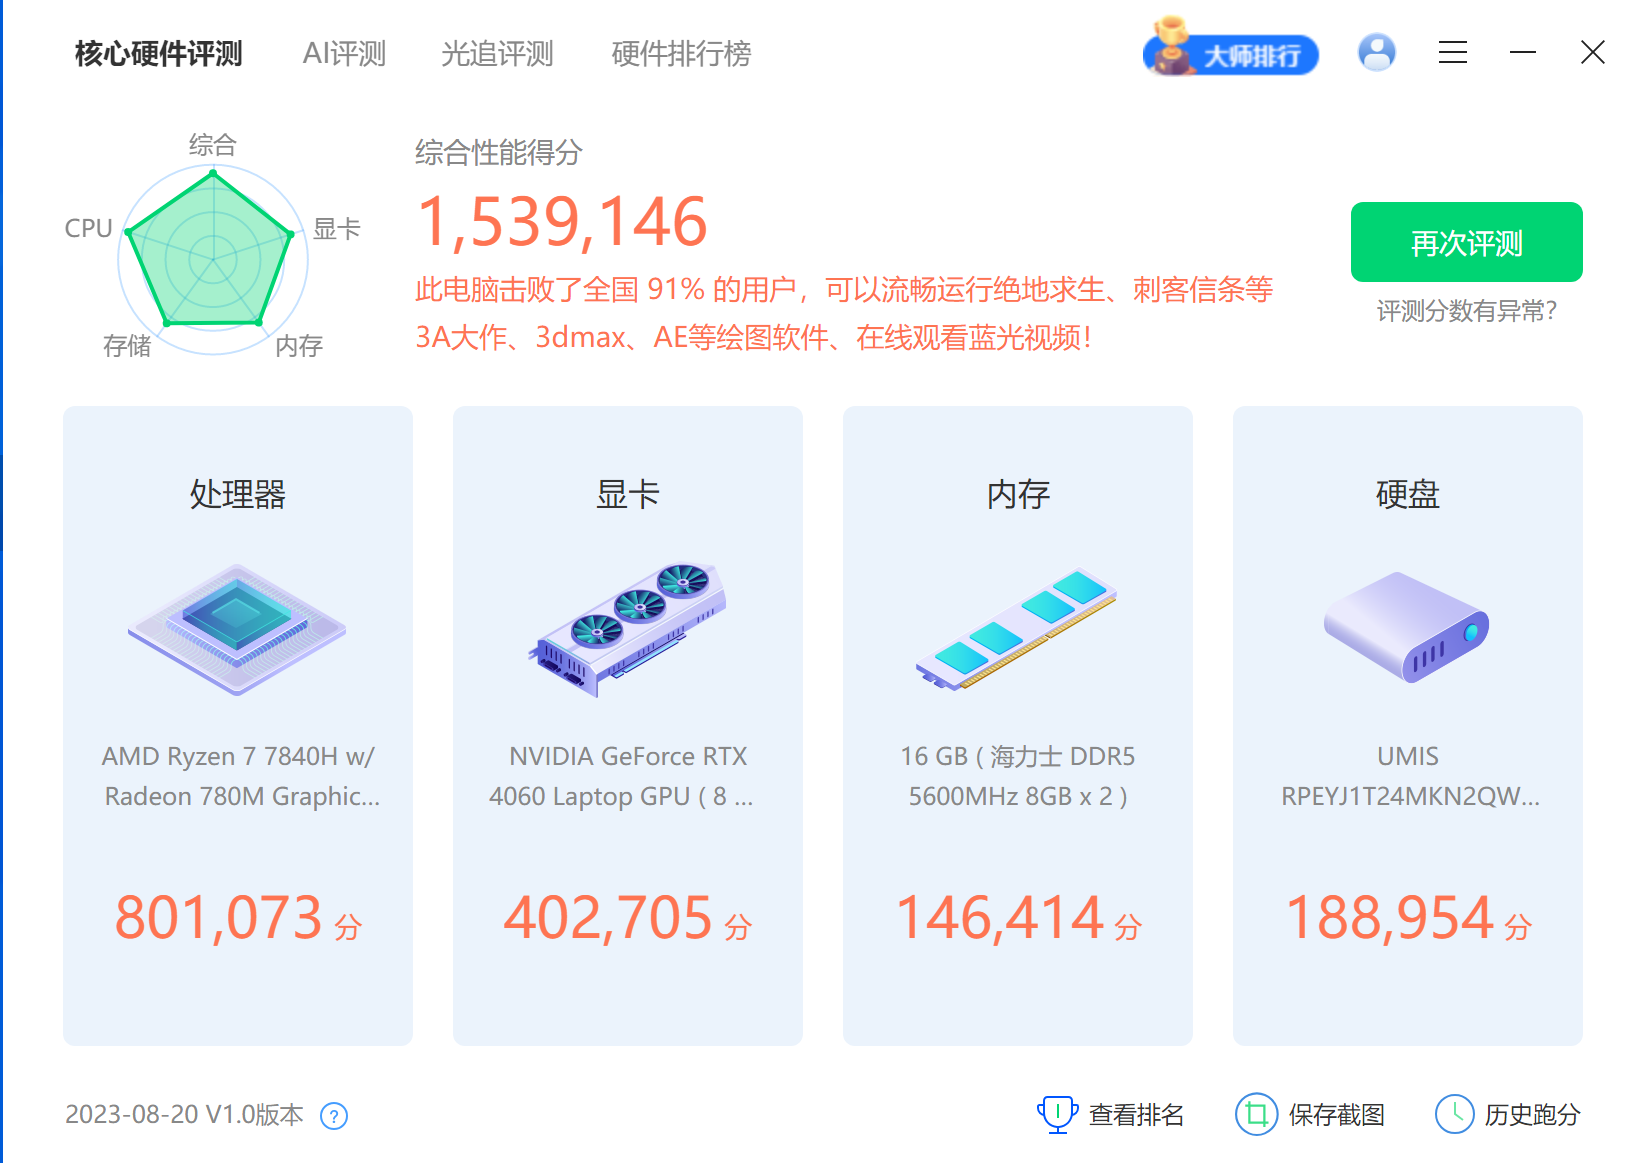
\includegraphics[width=0.9\linewidth]{2.png}
  \caption{Python 日志记录器}
   \end{figure}

\begin{figure}[H]
  \centering
    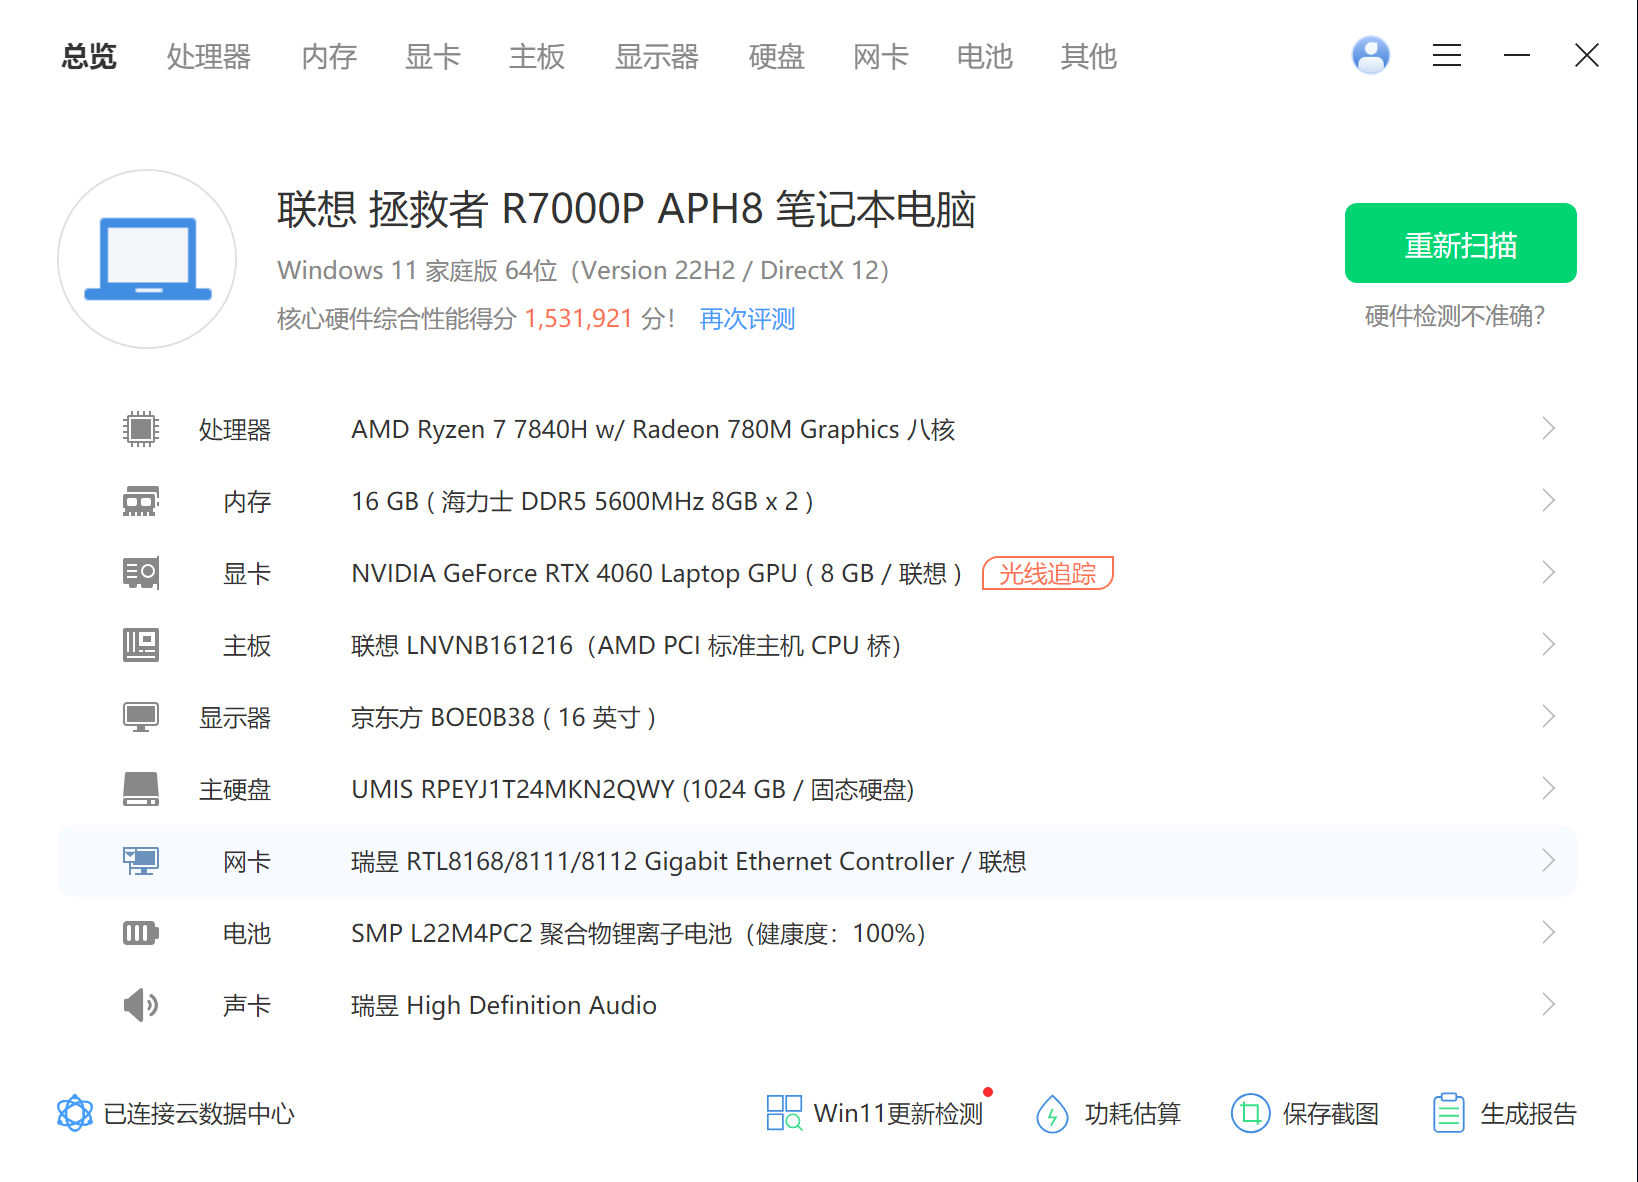
\includegraphics[width=0.9\linewidth]{3.png}
  \caption{运行结果}
   \end{figure}

\begin{figure}[H]
  \centering
    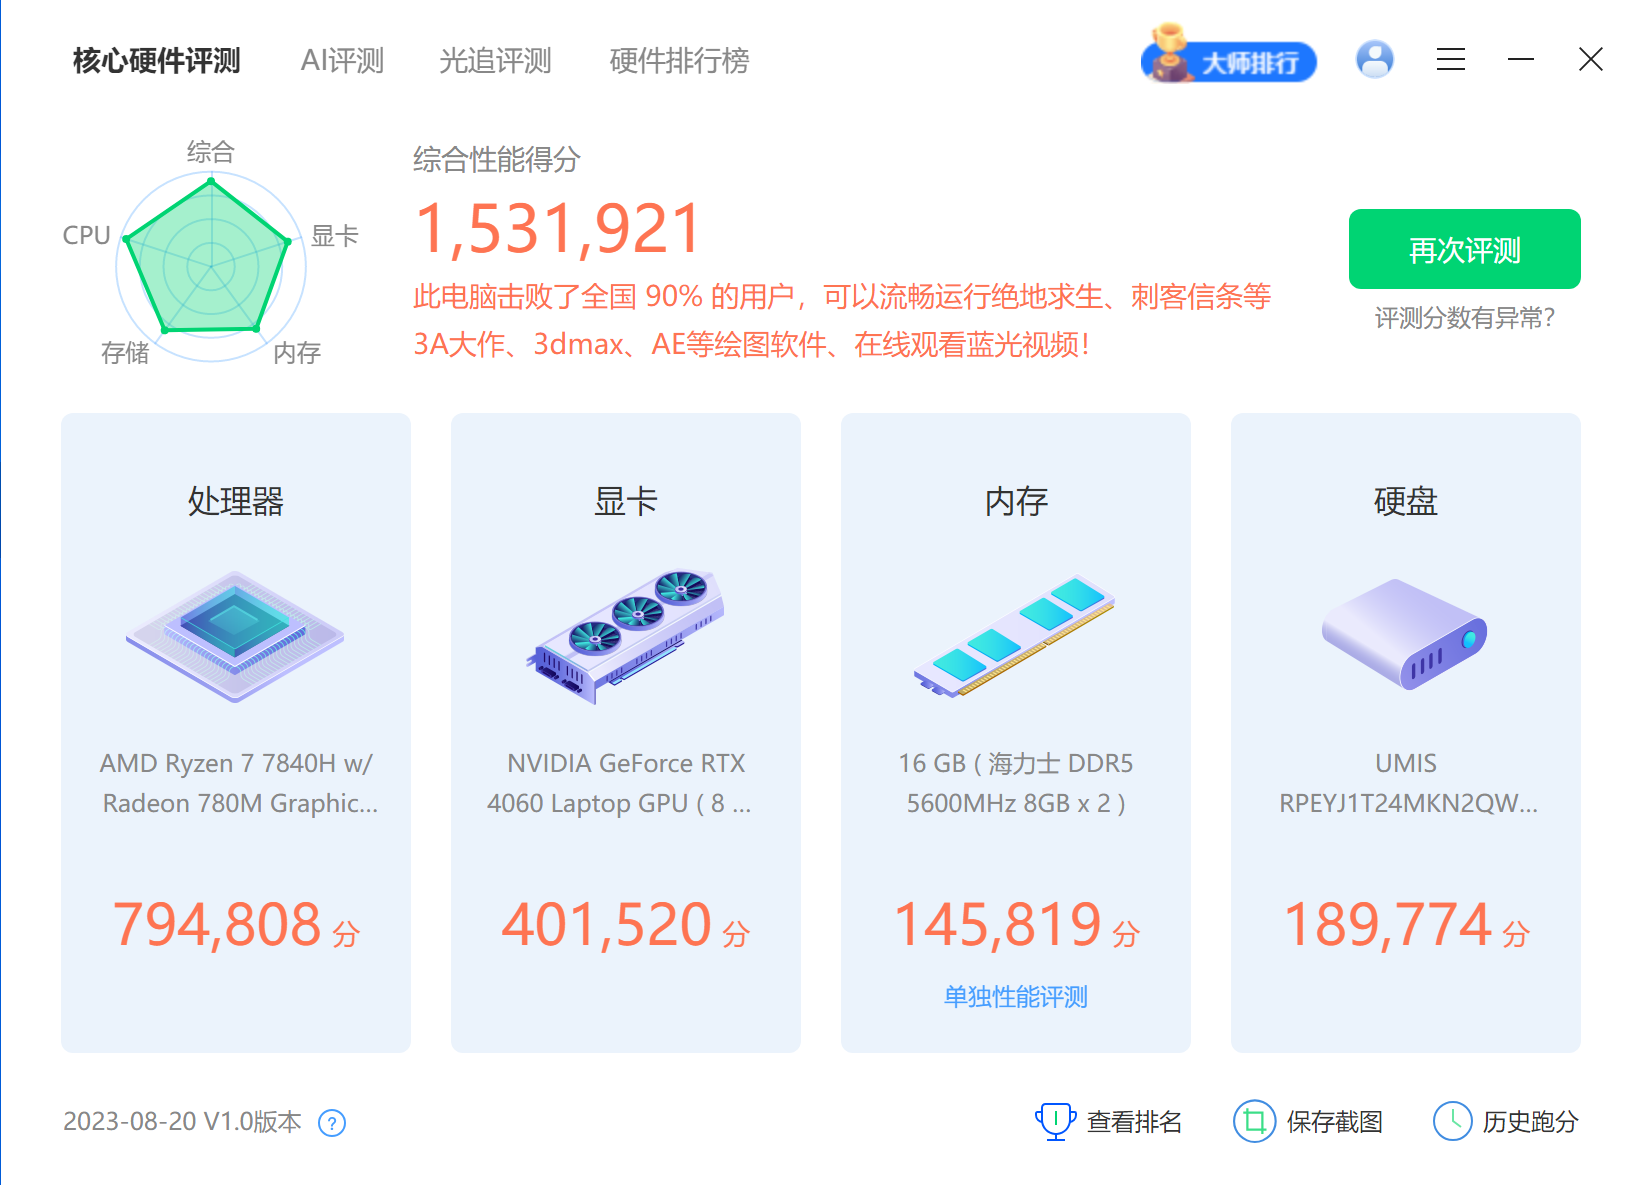
\includegraphics[width=0.9\linewidth]{4.png}
  \caption{运行结果}
   \end{figure}
   
   \begin{figure}[H]
  \centering
    \includegraphics[width=0.9\linewidth]{5.png}
  \caption{运行结果}
   \end{figure}
   
\subsection{调试器}  

当通过打印已经不能满足调试需求时,应该使用调试器。
调试器是一种可以允许我们和正在执行的程序进行交互的程序,它可以做到:
当到达某一行时将程序暂停;
一次一条指令地逐步执行程序;
程序崩溃后查看变量的值;
满足特定条件时暂停程序;
其他高级功能。
很多编程语言都有自己的调试器。Python 的调试器是 pdb.
下面对 pdb 支持的命令进行简单的介绍:

\begin{itemize}
  \item \texttt{l(ist)}    - 显示当前行附近的 11 行或继续执行之前的显示;
   \item \texttt{s(tep) }   - 执行当前行,并在第一个可能的地方停止;
  \item \texttt{n(ext) }   - 继续执行直到当前函数的下一条语句或者 return 语句;
  \item \texttt{b(reak)}   - 设置断点(基于传入的参数);
 \item \texttt{p(rint)}   - 在当前上下文对表达式求值并打印结果。还有一个命令是 pp ,它使用 pprint 打印;
 \item \texttt{r(eturn)}  - 继续执行直到当前函数返回;
 \item \texttt{q(uit)}  - 退出调试器。
  \end{itemize}

1. 在代码中插入断点
可以在代码中插入断点来启动调试器。常用的方法是在需要开始调试的地方插入以下代码:
import pdb; pdb.set\_trace()

2. 启动 Python 程序进行调试
也可以直接使用 pdb 来运行 Python 脚本,而不是插入断点。运行命令如下:
python -m pdb your\_script.py

\begin{figure}[H]
  \centering
    \includegraphics[width=0.9\linewidth]{6.png}
  \caption{使用pdb进行调试}
   \end{figure}
   

\subsection{使用shellcheck进行脚本分析}  

安装 shellcheck 并尝试对下面的脚本进行检查。这段代码有什么问题吗?请修复相关问题。在您的编辑器中安装一个linter插件,这样它就可以自动地显示相关警告信息。
\begin{lstlisting}
#!/bin/sh
## Example: a typical script with several problems
for f in $(ls *.m3u)
do
  grep -qi hq.*mp3 $f \
    && echo -e 'Playlist \$f contains a HQ file in mp3 format'
done
\end{lstlisting}
\begin{lstlisting}
在 Vim 中安装 neomake 和 shellcheck
打开 ~/.vimrc 文件,添加以下内容来集成 neomake 和 shellcheck:
vim

call plug#begin()
Plug 'neomake/neomake'
call plug#end()
然后在 Vim 中使用 :PlugInstall 安装插件。
安装完成后,可以通过以下命令安装 shellcheck:
bash
复制代码
sudo apt install shellcheck
最后,在编辑 shell 脚本时,neomake 将自动调用 shellcheck 进行静态分析并显示警告。
通过这种方式,你可以在 Vim 中实时看到 shellcheck 给出的代码问题。
\end{lstlisting}

安装完shellcheck后对脚本进行分析

\begin{figure}[H]
  \centering
    \includegraphics[width=0.9\linewidth]{7.png}
  \caption{报错结果}
   \end{figure}

\begin{lstlisting}
使用 shellcheck 对脚本进行检查,会发现以下问题:

使用 ls 和 for 的问题: $(ls *.m3u) 不推荐这样使用,因为它在处理带有空格或特殊字符的文件名时容易出错。应直接使用 for f in *.m3u。
echo -e 的问题: echo 的 -e 选项在 sh 中可能并不被所有平台支持,建议改为 printf,更为兼容。
$f 在字符串中没有被正确展开: $f 需要用双引号引起来,防止文件名中包含空格或特殊字符时出错。
\end{lstlisting}

\begin{lstlisting}
修复后的代码

#!/bin/sh
## Example: a typical script with several problems
for f in *.m3u
do
  grep -qi 'hq.*mp3' "$f" \
    && printf 'Playlist %s contains a HQ file in mp3 format\n' "$f"
done
\end{lstlisting}

\subsection{使用 cProfile分析排序性能} 
这里 有一些排序算法的实现。请使用 cProfile 和 line\_profiler 来比较插入排序和快速排序的性能。两种算法的瓶颈分别在哪里?然后使用 memory\_profiler 来检查内存消耗,为什么插入排序更好一些?然后再看看原地排序版本的快排。附加题:使用 perf 来查看不同算法的循环次数及缓存命中及丢失情况。

\begin{figure}[H]
  \centering
    \includegraphics[width=0.9\linewidth]{8.png}
  \caption{分析结果}
   \end{figure}

   \begin{figure}[H]
  \centering
    \includegraphics[width=0.9\linewidth]{9.png}
  \caption{分析结果}
   \end{figure}
   
\subsection{使用lineprofiler分析排序性能} 
使用 line\_profiler进行分析,需要安装:
 pip install line\_profiler
然后为需要分析的函数添加装饰器 @profile,并执行:
 kernprof -l -v sorts.py

对排序进行分析
快速排序
  Total time: 0.490021 s
 File: sorts.py
 Function: quicksort at line 22
插入排序
  Total time: 1.33387 s
 File: sorts.py
 Function: insertionsort at line 11

 显然快速排序更快
 使用 memory\_profiler进行分析,需要安装:

 pip install memory\_profiler
同样需要添加@profile 装饰器。 


\section{元编程}
 \subsection{makefile等的安装} 
对于大多数系统来说,不论其是否包含代码,都会包含一个 “构建过程”。需要执行一系列操作,这一过程包含了很多步骤,很多分支。执行一些命令来生成图表,然后执行另外的一些命令生成结果,然后再执行其他的命令来生成最终的论文。
make 是最常用的构建系统之一

安装makefile
\begin{lstlisting}
如果ubuntu没有Makefile,需要安装时,执行下面命令:

         sudo apt install make

         sudo apt install make-guile
\end{lstlisting}

\begin{figure}[H]
  \centering
    \includegraphics[width=0.9\linewidth]{10.png}
  \caption{安装成功}
   \end{figure}

python代码报错,没有matplotib库
\begin{figure}[H]
  \centering
    \includegraphics[width=0.9\linewidth]{11.png}
  \caption{报错信息}
   \end{figure}
   
 \subsection{使用makefile} 
安装Latex发行版将.tex文件转化为pdf文件
sudo apt update
sudo apt install texlive

\begin{figure}[H]
  \centering
\includegraphics[width=0.9\linewidth]{13.png}
  \caption{Latex的安装}
   \end{figure}
   
\begin{figure}[H]
  \centering
\includegraphics[width=0.9\linewidth]{12.png}
  \caption{Makefile}
   \end{figure}

接着使用make命令通过makefile生成pdf文件
\begin{figure}[H]
  \centering
\includegraphics[width=0.9\linewidth]{14.png}
  \caption{Makefile}
   \end{figure}
   
   \begin{figure}[H]
  \centering
\includegraphics[width=0.9\linewidth]{15.png}
  \caption{生成结果}
   \end{figure}
   
  \subsection{clean的使用}  
   大多数的 makefiles 都提供了 一个名为 clean 的构建目标,我们可以使用它清理文件,让 make 重新构建,“撤销”所有构建步骤。在上面的 makefile 中为paper.pdf实现一个clean 目标。
\begin{lstlisting}
git ls-files -o | xargs rm -f 
可以列出没有被 git 追踪的文件,一般是构建的中间产物,当然,需要首先设置 git 的忽略规则。
\end{lstlisting}


也可以使用另一种方式清理git仓库
将所有untracked文件移动到Untrack目录下
\begin{figure}[H]
  \centering
\includegraphics[width=0.9\linewidth]{16.png}
  \caption{设置git忽略该目录,用来放置untracked文件}
   \end{figure}

   
\subsection{Rust的构建系统的依赖管理}  
在 Rust 中,依赖管理是通过 Cargo.toml 文件完成的,里面可以指定依赖的版本。Rust 的版本管理语法使得开发者可以灵活控制依赖的版本。以下是每种语法的解释和实际应用场景。
1. 尖号 (\^) 版本要求
尖号语法是 Rust 依赖管理的默认方式。它允许更新到不改变主要版本的最新版本(语义化版本中的 major 版本)。
场景:
假设我们依赖一个库 rand,版本 0.8.3,可以指定如下:

[dependencies]
rand = "\^0.8.3"
意义:这意味着项目可以使用 rand 版本 0.8.x,但不允许自动升级到 1.x.x。这样可以确保不引入破坏性的更改,保持与当前代码兼容。

2. 波浪号 (~) 版本要求
波浪号语法指定版本号的最小更改。它允许升级到不改变次版本号的补丁版本。

场景:
假设依赖的库 serde,版本 1.0.64,我们可以这样指定:

[dependencies]
serde = "~1.0.64"
意义:这个语法允许项目升级 serde 到 1.0.x 的任何补丁版本,如 1.0.99,但不会允许升级到 1.1.x。这种用法适合依赖于特定功能且希望获取补丁更新但不改变 API 的情况。

3. 通配符 (*) 版本要求
通配符允许高度的灵活性,通常用于快速原型开发时,不介意升级到最新的主要或次要版本。

场景:
如果我们只关心使用最新的 regex 包,而不关心版本兼容性,可以使用如下语法:

[dependencies]
regex = "1.*"
意义:允许使用 regex 库的任何 1.x.x 版本。这适合在开发早期阶段使用最新的功能和性能改进,但风险在于未来的主要版本可能引入不兼容更改。
\begin{figure}[H]
  \centering
    \includegraphics[width=0.9\linewidth]{17.png}
  \caption{Cargo.toml文件结构}
   \end{figure}   

   \begin{figure}[H]
  \centering
    \includegraphics[width=0.9\linewidth]{10.png}
  \caption{运行结果}
   \end{figure}   

\section{Pytorch编程}


\subsection{环境配置}

安装 PyTorch
可以通过以下命令安装 PyTorch:

pip install torch torchvision torchaudio

安装 torch库
pip install torch torchvision torchaudio

安装 humpy
\begin{figure}[H]
  \centering
    \includegraphics[width=0.9\linewidth]{18.png}
  \caption{安装成功}
   \end{figure}  

   
\subsection{张量和自动求导}
 张量(Tensor)
张量是 PyTorch 的核心数据结构,类似于 NumPy 的数组,但支持 GPU 加速。创建张量的示例
\begin{lstlisting}
  import torch

# 创建一个 2x3 的张量,元素为随机数
x = torch.rand(2, 3)

# 创建一个 2x3 的全零张量
zeros = torch.zeros(2, 3)

# 创建一个 2x3 的全一张量
ones = torch.ones(2, 3)

# 打印张量的值
print(x)
print(zeros)
print(ones)
\end{lstlisting}

\begin{figure}[H]
  \centering
    \includegraphics[width=0.5\linewidth]{19.png}
  \caption{运行结果}
   \end{figure}  
   
自动求导
PyTorch 提供了 autograd 模块来自动计算梯度。要使用自动求导,需要将 requires\_grad 设置为 True:

\begin{lstlisting}
import torch

# 创建一个张量,并设置 requires_grad=True
try:
    x = torch.tensor([1.0, 2.0, 3.0], requires_grad=True)

    # 定义一个简单的操作并计算梯度
    y = x * 2
    y.mean().backward()
    
    # 打印梯度
    print(x.grad)
except Exception as e:
    print(f"发生错误: {e}")
    
\end{lstlisting}

\begin{figure}[H]
  \centering
\includegraphics[width=0.9\linewidth]{20.png}
  \caption{运行结果}
   \end{figure}  


   
\subsection{创建模型}
在 PyTorch 中,你可以使用 torch.nn.Module 创建自定义模型。以下是一个简单的神经网络模型的示例:

\begin{verbatim}
import torch
import torch.nn as nn
import torch.optim as optim

# 一个简单的前馈神经网络模型
class SimpleModel(nn.Module):
    # 初始化模型的层
    def __init__(self):
        super(SimpleModel, self).__init__()
        self.fc1 = nn.Linear(10, 5)  # 第一层全连接层
        self.fc2 = nn.Linear(5, 1)    # 第二层全连接层

    # 定义模型的前向传播过程
    def forward(self, x):
        x = torch.relu(self.fc1(x))  # 在第一层后应用ReLU激活函数
        x = self.fc2(x)               # 从第二层输出
        return x

# 实例化模型
model = SimpleModel()

# 生成随机的输入数据
input_data = torch.randn(1, 10)  # 创建一个大小为(1, 10)的随机输入

# 将输入数据传递给模型
output = model(input_data)

# 打印输出结果
print(output)
  \end{verbatim}

这个模型是一个简单的前馈神经网络,主要用于处理特征维度为10的输入数据,并将其映射到一个输出值。具体来说,该模型可以用于以下场景:

回归任务:由于模型的输出层只有一个神经元,适合用于输出一个连续值,例如预测房价、温度等。

特征学习:这个模型可以用于学习输入特征的表示,进而在后续的任务中(例如分类或回归)使用。

调试和学习工具:作为一个简单的神经网络示例,它有助于理解前馈网络的基本结构和前向传播过程。

总的来说,该模型是一个基础的深度学习模型,用于学习和预测的任务。

\subsection{数据加载}
PyTorch 提供了 torch.utils.data.DataLoader 用于加载数据。以下是一个简单的数据加载示例:

\begin{verbatim}
  import torch
from torch.utils.data import DataLoader, TensorDataset
try:
    # 创建一些数据
    x_data = torch.randn(100, 10)
    y_data = torch.randn(100, 1)

    # 检查数据的形状是否一致
    if x_data.shape[0] != y_data.shape[0]:
        raise ValueError("x_data 和 y_data 的样本数量不一致。")

    # 创建数据集
    dataset = TensorDataset(x_data, y_data)

    # 创建数据加载器
    dataloader = DataLoader(dataset, batch_size=32, shuffle=True)

    # 迭代数据
    for x_batch, y_batch in dataloader:
        # 进行训练
        pass

except Exception as e:
    print(f"发生错误: {e}")

  \end{verbatim}

  
\subsection{训练、保存和加载模型}
以下是一个简单的训练循环:


\begin{figure}[H]
  \centering
\includegraphics[width=0.9\linewidth]{21.png}
  \caption{训练模型的代码}
   \end{figure}  


保存和加载模型的代码示例如下:

\begin{verbatim}
  # 保存模型
torch.save(model.state_dict(), 'model.pth')

# 加载模型
model = SimpleModel()
model.load_state_dict(torch.load('model.pth'))
  \end{verbatim}



 \section{大杂烩}
\subsection{修改键位映射}
键盘是主要输入工具。它像计算机里的其他部件一样是可配置的,一个很常见的配置是修改键位映射。通常这个功能由在计算机上运行的软件实现。当某一个按键被按下,软件截获键盘发出的按键事件(keypress event)并使用另外一个事件取代。比如:
将 Caps Lock 映射为 Ctrl 或者 Escape:Caps Lock 使用了键盘上一个非常方便的位置而它的功能却很少被用到,所以我们非常推荐这个修改;
将 PrtSc 映射为播放/暂停:大部分操作系统支持播放/暂停键;
交换 Ctrl 和 Meta 键(Windows 的徽标键或者 Mac 的 Command 键)。
\begin{figure}[H]
  \centering
    \includegraphics[width=0.9\linewidth]{22.png}
  \caption{修改键位映射的工具}
   \end{figure}  
   
   \begin{figure}[H]
  \centering
    \includegraphics[width=0.9\linewidth]{23.png}
  \caption{将不常用的大小写键改为Enter键}
   \end{figure}  


   
 

\subsection{Markdow进行文字段落操作}
职业生涯中大概率会编写各种各样的文档。在很多情况下这些文档需要使用标记来增加可读性,比如:插入粗体或者斜体内容,增加页眉、超链接、以及代码片段。
在不使用 Word 或者 LaTeX 等复杂工具的情况下,可以使用 Markdown 这个轻量化的标记语言(markup language)。很多环境都支持并使用 Markdown 的一些子功能。

\begin{verbatim}
用 * 包围的文字表示强调(斜体),或者用 ** 表示特别强调(粗体);
以 # 开头的行是标题,# 的数量表示标题的级别,比如:##二级标题;
以 - 开头代表一个无序列表的元素。一个数字加 .(比如 1.)代表一个有序列表元素;
反引号 `(backtick)包围的文字会以 代码字体 显示。如果要显示一段代码,可以在每一行前加四个空格缩进,或者使用三个反引号包围整个代码片段:

如果要添加超链接,将 需要显示 的文字用方括号包围,并在后面紧接着用圆括号包围链接:[显示文字](指向的链接)。
  \end{verbatim}


绘制图像的例子
  \begin{figure}[H]
  \centering
    \includegraphics[width=0.9\linewidth]{24.png}
  \caption{markdown的源码}
   \end{figure}  
   
 

  \begin{figure}[H]
  \centering
    \includegraphics[width=0.9\linewidth]{26.png}
  \caption{markdown的生成结果}
   \end{figure}  

   
\subsection{使用markdown插入链接和图片}
\begin{verbatim}
1. 链接
创建链接的基本语法是 [链接文本](URL)。
[实例链接](https://www.example.com)
2. 图片
插入图片的基本语法是 ![替代文本](图片URL)。
![示例图片](https://via.placeholder.com/150)
可以使用网站式的绝对链接和本地式的相对链接((D:\class python code\example.png)
\end{verbatim}

\subsection{使用markdown插入代码和引用}

\begin{verbatim}
3. 代码
行内代码
使用反引号 ` 包围代码片段。

这是 `行内代码` 示例。
代码块
使用三个反引号 ``` 来包围代码块,可以指定语言来进行语法高亮。

```python
def hello\_world():
    print("Hello, world!")
shell

4. 引用
使用 `>` 来创建块引用。

```markdown
> 这是一个引用块。
> 
> 可以用于引用别人的话。
\end{verbatim}

\subsection{使用markdown插入分割线、表格和任务列表}
\begin{verbatim}
5. 分隔线
使用三个或更多的星号 *、减号 - 或下划线 _ 来创建分隔线。

***
---
___
6. 表格
使用管道符号 | 和减号 - 来创建表格。

markdown
复制代码
| 列 1 | 列 2 | 列 3 |
|------|------|------|
| 单元格 1 | 单元格 2 | 单元格 3 |
| 单元格 4 | 单元格 5 | 单元格 6 |
7. 任务列表
使用 - [ ] 来创建任务列表项。

markdown
复制代码
- [x] 完成任务 1
- [ ] 任务 2
- [ ] 任务 3
\end{verbatim}


\begin{figure}[H]
  \centering
    \includegraphics[width=0.9\linewidth]{25.png}
  \caption{markdown的源码}
   \end{figure}
    \begin{figure}[H]
  \centering
\includegraphics[width=0.9\linewidth]{27.png}
  \caption{markdown的生成结果}
   \end{figure} 

 \section{遇到的问题和学到的经验}

\subsection{问题描述:}
在进行基本的张量操作时遇到困难,比如张量的创建、操作和维度变换。在定义和训练模型时遇到了挑战,比如如何定义网络架构、如何设置损失函数和优化器、以及如何执行训练循环。对如何使用 PyTorch 的自动求导功能进行梯度计算感到困惑。
  \subsection{学到的经验}
张量操作:
学会了如何创建和操作 PyTorch 张量,包括基础的数学操作和维度变换。
模型构建和训练:
掌握了如何定义和训练神经网络模型,包括如何构建模型架构、设置损失函数和优化器,以及编写训练循环。
自动求导:
了解了如何使用 PyTorch 的自动求导功能来计算梯度,以及如何在训练过程中应用梯度更新。
数据加载:
学会了如何使用 DataLoader 和 Dataset 来高效地加载和预处理数据,为模型训练做好准备。
模型保存和加载:
掌握了如何保存和加载训练好的模型,以便在之后的时间点进行推断或继续训练。
 \subsection{问题描述:}
 找不到 kernprof 命令
执行 kernprof 命令时提示 “command not found”。PyTorch 模块导入错误
尽管安装了 PyTorch,但运行脚本时仍然出现 ModuleNotFoundError: No module named 'torch'。
  \subsection{学到的经验}
安装 line\_profiler 包,该包提供了 kernprof 命令。可以通过以下命令安装:
pip install line\_profiler
安装完成后,重新运行 kernprof 命令进行性能分析。解决方法: 确认 pip 安装路径与 Python 解释器匹配。检查 sys.executable 输出,确保 pip 安装的路径在 Python 环境的 site-packages 中。如果路径不匹配,考虑重新安装 PyTorch:解决方法: 安装 LaTeX 相关工具。可以通过以下命令安装 texlive:
sudo apt install texlive
 \subsection{问题描述:}在尝试使用命令行安装Python库(如使用pip)时,经常遇到权限问题或路径错误,导致安装失败。
 \subsection{学到的经验}
  学会了使用sudo(在Linux/macOS上)或管理员命令提示符(在Windows上)来提升权限,以及使用虚拟环境(如venv或conda)来隔离和管理不同项目的依赖。
 \subsection{问题描述:}Python基础语法混淆:在编写Python脚本时,经常混淆变量作用域、列表和元组的区别,以及循环和条件语句的嵌套。
\subsection{学到的经验}通过大量练习和阅读官方文档,加深了对Python基础语法的理解,学会了使用调试工具(如pdb)来追踪和解决问题。

\subsection{问题描述:}
pdflatex 命令未找到
在运行 make 命令时提示 pdflatex: command not found。
脚本中存在语法错误
 Shell 脚本使用 ls 和 for 导致问题,且 echo -e 在某些环境中不可用。
\subsection{解决方法:}
 修改脚本为更兼容的格式

\subsection{学到的经验}
学到的经验总结
持续学习:技术日新月异,保持对新技术和新方法的关注和学习是非常重要的。
实践出真知:理论知识是基础,但只有通过实践才能真正掌握和应用。
社区资源:充分利用官方文档、社区论坛和开源项目等资源,可以更快地解决问题并提升技能。
耐心和毅力:面对问题和挑战时,保持耐心和毅力是成功的关键。

 \section{代码链接}
      请访问以下链接来查看我在Github上的相关练习、报告和代码:
\url{https://github.com/boken319/git_push}
我的在线Latex文件的网址:
\url{https://cn.overleaf.com/read/zjnsjqsmtcgf#239a34}

\end{document}
